\chapter{Carga de datos para analítica}
Para llevar los datos a Athena se usan tres contenedores Python. \texttt{ingesta-catalogo} extrae tablas de PostgreSQL, \texttt{ingesta-comunity} extrae tablas de MySQL y \texttt{ingesta-iteraction} extrae colecciones de MongoDB. Cada proceso genera archivos CSV en UTF-8, limpia los saltos de línea y los carga con \texttt{boto3} en un bucket S3 configurable.
\begin{table}[H]\centering\small\caption{Datos extraídos hacia S3}\begin{tabularx}{\textwidth}{p{.25\textwidth}p{.2\textwidth}X}\toprule Origen&Prefijo S3&Datos\\\midrule Catalog/PostgreSQL&\path{resultados/catalogo}&Películas, artistas, géneros, relaciones, videos y subtítulos.\\Community/MySQL&\path{resultados/comunity}&Usuarios, clubes, membresías, salas y participantes.\\Interaction/MongoDB&\path{resultados/iteraction}&Colecciones disponibles, incluidas reseñas, likes y watchlists.\\\bottomrule\end{tabularx}\end{table}
Los archivos se guardan con la entidad y la fecha \texttt{YYYY-MM-DD}. Así, Glue puede registrar su estructura y Athena puede consultarlos sin cargar las bases de datos principales. La ejecución periódica y los procesos de Glue que detectan esa estructura se configuran al desplegar esta parte de la solución.

\section*{Evidencia de catalogación con AWS Glue}
Para registrar la estructura de los archivos almacenados en S3 se configuró el crawler \texttt{astra-crawler} en AWS Glue. El crawler utiliza como fuente \path{s3://cloud-astra-movies/resultados/} y registra los metadatos en la base \texttt{astra\_analytics}. La ejecución mostrada finalizó correctamente (\texttt{Succeeded}) y registró la creación de 13 tablas. Estas tablas quedan disponibles para las consultas realizadas posteriormente mediante Amazon Athena.
\begin{figure}[H]
\centering
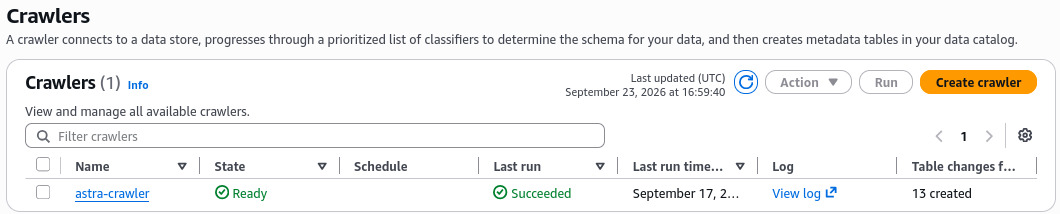
\includegraphics[width=.96\textwidth]{evidence/glue/athena_crawler1.jpeg}
\caption{Ejecución del crawler \texttt{astra-crawler} en AWS Glue, con 13 tablas creadas.}
\label{fig:glue-crawler-run}
\end{figure}
\begin{figure}[H]
\centering
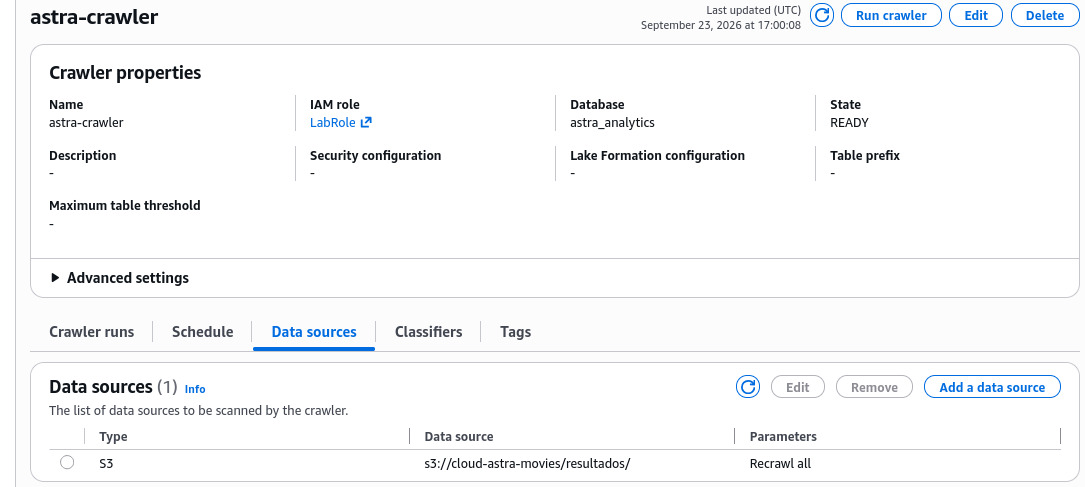
\includegraphics[width=.96\textwidth]{evidence/glue/athena_crawler2.jpeg}
\caption{Configuración del crawler \texttt{astra-crawler} con origen en Amazon S3 y destino en la base \texttt{astra\_analytics}.}
\label{fig:glue-crawler-properties}
\end{figure}
